\documentclass{article}
\usepackage[utf8]{inputenc}
\usepackage[T1]{fontenc}

% les packages
\usepackage[english]{babel}
\usepackage{graphicx}
%\usepackage{wrapfig}
%\usepackage{floatrow}
%\usepackage{sistyle}
%\usepackage{prettyref}
\usepackage{graphicx}
%\usepackage{dcolumn}
\usepackage{bm}
\usepackage{amsmath}
\usepackage{amssymb}
%\usepackage{SIunits}
%\usepackage{times}
\usepackage{color}

%\usepackage{float}
%\usepackage{a4}

%\usepackage{ae,aecompl,aeguill} %Pour avoir de jolies polices avec pdf.
%\usepackage{pslatex}
%\usepackage{makeidx}
\usepackage{hyperref}

\usepackage{tikz}
\usetikzlibrary{arrows}
\usepackage{tikzorbital}
\usepackage{tikz-3dplot}
\usepackage{apacite}

\newcommand*{\doi}{}
\makeatletter
\newcommand{\doi@}[1]{\href{https://doi.org/#1}{#1}}
\DeclareRobustCommand{\doi}{\hyper@normalise\doi@}
\makeatother

% les formats

\setlength{\textwidth}{17cm}
\setlength{\textheight}{23cm}
\setlength{\evensidemargin}{0cm}
\setlength{\oddsidemargin}{0cm}
\definecolor{Highlight}{cmyk}{0.0,0.89,0.94,0.1}
\newcommand\High{\color{Highlight}}


% les définitions

\def\N{\mbox{I\hspace{-.15em}N}}% entiers naturels
\def\Z{\mbox{Z\hspace{-.3em}Z}}%
\def\R{\mbox{I\hspace{-.15em}R}}
\def\C{\mbox{l\hspace{-.47em}C}}
\def\Q{\mbox{l\hspace{-.47em}Q}}
\def\P{\mbox{I\hspace{-.15em}P}}
\def\E{\mbox{I\hspace{-.15em}E}}
\def\pp{ \|}
\def\ii{\^{\i}}
\newcommand{\bra}[1]{\langle #1|}
\newcommand{\ket}[1]{|#1\rangle}
\newcommand{\braket}[2]{\langle #1|#2\rangle}
\newcommand{\op}[1]{\hat{#1}}
\def\build#1_#2^#3{\mathrel{\mathop{\kern 0pt#1}\limits_{#2}^{#3}}}


\title{Tight-Binding formalism}
\author{Cyrille Barreteau }
\date{\today}

\begin{document}
\vspace{-2cm}
\maketitle


\begin{figure}[!ht]
\begin{center}
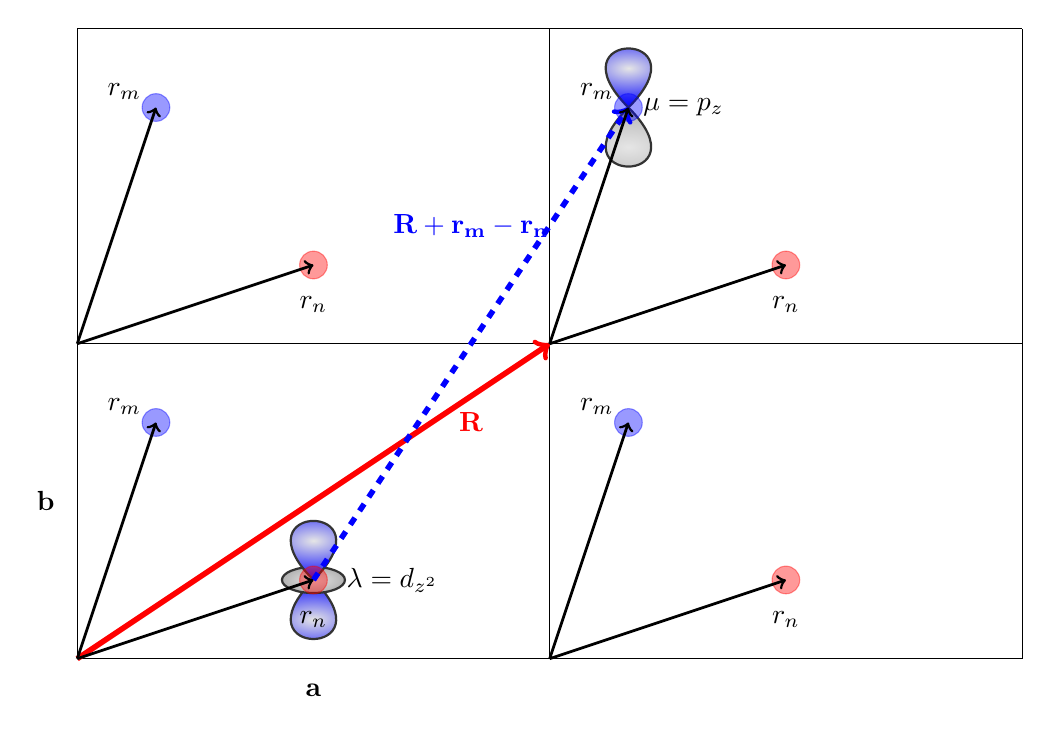
\begin{tikzpicture}
\draw  (0,0)-- (12,0);
\draw  (0,0)-- (0,8);
\draw  (0,8)-- (12,8);
\draw  (12,0)-- (12,8);
\draw  (0,4)-- (12,4);
\draw  (6,0)-- (6,8);

\draw[color=blue,fill=blue,opacity=0.4]  (1,3) circle (5pt);
\draw[color=red,fill=red,opacity=0.4]    (3,1) circle (5pt);

\draw[color=blue,fill=blue,opacity=0.4]  (7,7) circle (5pt);
\draw[color=red,fill=red,opacity=0.4]    (9,5) circle (5pt);

\draw[color=blue,fill=blue,opacity=0.4]  (1,7) circle (5pt);
\draw[color=red,fill=red,opacity=0.4]    (3,5) circle (5pt);

\draw[color=blue,fill=blue,opacity=0.4]  (7,3) circle (5pt);
\draw[color=red,fill=red,opacity=0.4]    (9,1) circle (5pt);

\draw [->,line width=2pt,color=red] (0,0) -- (6,4);
\draw [->,line width=2pt,color=blue, dashed] (3,1) -- (7,7);
\draw [->,line width=1pt] (0,0) -- (1,3);
\draw [->,line width=1pt] (0,0) -- (3,1);
\draw [->,line width=1pt] (6,4) -- (7,7);
\draw [->,line width=1pt] (6,4) -- (9,5);
\draw [->,line width=1pt] (0,4) -- (1,7);
\draw [->,line width=1pt] (0,4) -- (3,5);
\draw [->,line width=1pt] (6,0) -- (7,3);
\draw [->,line width=1pt] (6,0) -- (9,1);

\draw (3,-0.4) node {$\mathbf{a}$};
\draw (-0.4,2) node {$\mathbf{b}$};

\draw (0.6,3.2) node {$r_m$};
\draw (3,0.5) node {$r_n$};
\draw (6.6,7.2) node {$r_m$};
\draw (9,4.5) node {$r_n$};
\draw (6.6,3.2) node {$r_m$};
\draw (9,0.5) node {$r_n$};
\draw (0.6,7.2) node {$r_m$};
\draw (3,4.5) node {$r_n$};

%\draw (2.5,1) ellipse (0.5cm and 0.25cm);
%\draw (3.5,1) ellipse (0.5cm and 0.25cm);
%\draw[color=red] (3.5,1) node {$\lambda$};

% \draw (7,6.5) ellipse (0.25cm and 0.5cm);
% \draw (7,7.5) ellipse (0.25cm and 0.5cm);
% \draw[color=blue] (7,7.5) node {$\mu$};
 
\draw[color=red] (5,3) node {$\mathbf{R}$};
\draw[color=blue] (5,5.5) node {$\mathbf{R+r_m-r_n}$};

    % Figure Eight Curve
%    \draw[domain   = 0:360,
%          samples  = 200,
%          variable = \t,
%          smooth, blue, thick]
%    plot ({2*cos(\t)},{2*sin(2*\t)});

\orbital[pos = {(3,1)}]{dz2}
\draw (4,1) node {$\lambda=d_{z^2}$};

\orbital[pos = {(7,7)}]{pz}
\draw (7.7,7) node {$\mu=p_z$};

\end{tikzpicture}
\caption{\sl geometry of the unit-cell and its periodicity}
\label{fig:geom}
\end{center}
\end{figure}

\section{Notations}
Here are defined some notations that come from the reference \cite{barreteauEfficientMagneticTightbinding2016}.

\subsection{Geometry}
\label{sec:Geometry}
\noindent
Born von Karman (BVK) conditions are used.
The lattice parameters are $a,b$ and $c$.

\noindent
BVK: $L_a=N_a \times a$,\; $L_b=N_b \times b$,\; $L_c=N_c \times c$.

\noindent
Total number of cells: $N=N_a \times N_b \times N_c$

\noindent
Periodicity along lattice vectors $\mathbf a$, $\mathbf b$ et $\mathbf c$. 
Volume of the unit-cell : $\omega=\mathbf{a}.(\mathbf{b} \times \mathbf{c})$

$\mathbf{R}=n_a \mathbf{a}+n_b \mathbf{b}+n_c \mathbf{c}$.

\noindent
Reciprocal vectors  $\mathbf{a}^*$, $\mathbf{b}^*$ and $\mathbf{c}^*$. Volume of the Brillouin zone $\omega^*=\displaystyle{\frac{2\pi^3}{\omega}}$

$\mathbf{g}= h \mathbf{a}^*+k \mathbf{b}^*+l \mathbf{c}^*$.

\noindent
Scalar product between a real-space lattice vector and a reciprocal lattice vector: $\mathbf{R}.\mathbf{g}=2\pi(n_ah+n_bk+n_cl)$

\noindent
If $\mathbf{R} \in \text{Bravais lattice}$ and $\mathbf{g} \in \text{Reciprocal lattice}$ then $\mathbf{R}.\mathbf{g}=2\pi n \Rightarrow e^{i\mathbf{R}.\mathbf{g}}=1$

\noindent
Number of atoms in the unit-cell : $n_{\text at}$

\noindent
$\mathbf{R}, \mathbf{R}'$: periodic vectors of the Bravais lattice

\noindent $\mathbf{r}_n,\mathbf{r}_m$: position of the atoms in the unit-cell $n=1\cdots, n_{\text at}$.


\subsection{Orbitals}
\label{sec:orbitals}

\noindent
$\lambda, \mu, \nu$: orbitals 
$\ket{s},\ket{p_x},\ket{p_y},\ket{p_z},
\ket{d_{xy}},\ket{d_{yz}},\ket{d_{zx}},\ket{d_{x^2-y^2}},\ket{d_{3z^2-r^2}}$. $l$ orbitals.

\noindent
Atomic wave functions of orbital $\lambda$ centered on site $(R,n)$ .

\[\braket{\mathbf{r}}{R,n,\lambda} = \phi_{\lambda}(\mathbf{r}-\mathbf{R}-\mathbf{r}_n)\]




\subsection{Hamiltonian}

\noindent
$\op{H}$ Hamiltonian operator.

\noindent
$\bm{H}$ Hamiltonian matrix:

\noindent
\[ \displaystyle \bm{H}_{R,n,R',m}^{\lambda, \mu}=\bra{ R,n,\lambda} \op{H} \ket{ R',m,\mu } \quad ;\quad
\bm{S}_{R,n,R',m}^{\lambda, \mu}=\bra{ Rn,\lambda} \op{\mathbb{I}} \ket{R' m,\mu }\]
where $\op{\mathbb{I}}$ is the identity operator.


\section{Bloch Theorem}

\subsection{Notations}

\noindent $\ket{\alpha, \mathbf{k} }$ is a Bloch function of index
$\alpha$ ($\alpha=1, \cdots, n_{\text{at}} \times l$) and wave-vector $\mathbf{k}\in \text{1BZ}$


\noindent
  $ \mathbf{k}=  k_a \mathbf{a}^*+k_b \mathbf{b}^*+k_c \mathbf{c}^* \in \mbox{1BZ}
\quad k_{i=a,b,c}= (2\times n_i -N_i -1)/(2 N_i) \quad (n_i=1,\cdots,N_i)$ .

\noindent
We recall some relations:

\[ \frac{1}{N}\sum_{\mathbf{R}} e^{i\mathbf{k}.\mathbf{R}}=\delta_{\mathbf{k}} 
\quad ; \quad
\frac{1}{N^2}\sum_{\mathbf{R},\mathbf{R}'} 
e^{i(\mathbf{k}-\mathbf{k'}).(\mathbf{R}-\mathbf{R}')}=\delta_{\mathbf{k}, 
\mathbf{k}'} \]


\subsection{Bloch Functions}

\noindent
Expansion of wave functions on atomic orbitals

\[\displaystyle \ket{\Psi_{\alpha}}=\sum_{\mathbf{R},n,\lambda} C_{R n  \lambda}^{\alpha} \ket{\mathbf{R},n,\lambda }\]


\noindent
According to Bloch theorem, the functions that are solutions of the Schrödinger equations can be labeled by two indices $\alpha, \mathbf{k}$:

\[ \displaystyle C_{R,n \lambda}^{\alpha}=\frac{1}{\sqrt{N}}e^{i  \mathbf{k}.\mathbf{R}}e^{i \mathbf{k}.\mathbf{r}_n} C_{n \lambda}^{\alpha}(\mathbf{k})\]

\noindent
So:

\[\displaystyle \ket{\alpha, \mathbf{k}}=\sum_{n,\lambda} C_{n \lambda}^{\alpha}(\mathbf{k})
\frac{e^{i \mathbf{k}.\mathbf{r}_n}}{\sqrt{N}} \sum_{\mathbf{R}} e^{i \mathbf{k}.\mathbf{R}} \ket{\mathbf{R},n,\lambda } \]

\noindent Introducing a TB basis adapted to periodicity $|n,\lambda, \mathbf{k} \rangle$ one gets:

\[\displaystyle \ket{\alpha, \mathbf{k} }=\sum_{n,\lambda} C_{n \lambda}^{\alpha}(\mathbf{k})\ket{n,\lambda,\mathbf{k}}
\quad \mbox{with} \quad \displaystyle 
\ket{n,\lambda,\mathbf{k}}=\frac{e^{i \mathbf{k}.\mathbf{r}_n}}{\sqrt{N}} \sum_{\mathbf{R}} e^{i \mathbf{k}.\mathbf{R}} \ket{\mathbf{R},n,\lambda }\]

\noindent
The closure relation reads

\[\displaystyle \sum_{\alpha,\mathbf{k}} \ket{\alpha,\mathbf{k}}  \bra{\alpha,\mathbf{k}}=\op{\mathbb{I}}\]

\noindent
and the Hamiltonian:

\[ \sum_{\alpha,\mathbf{k}} \ket{\alpha,\mathbf{k}} \varepsilon_{\alpha}(\mathbf{k}) \bra{\alpha,\mathbf{k}}=\op{H}\]


\noindent
If the Bloch coefficient $C_{i \lambda}^{\alpha}(\mathbf{k})$ are normalized correctly:

\[ \braket{\alpha,\mathbf{k}}{\beta,\mathbf{k}}=
\sum_{n \lambda,m \mu} (C_{n \lambda}^{\alpha}(\mathbf{k}))^{\star} S_{a,b}^{\lambda,\mu}(\mathbf{k})C_{m \mu}^{\beta}(\mathbf{k})=\delta_{\alpha \beta}
\quad \forall \mathbf{k} \]


\section{Schr\"odinger Equation}

\noindent
Schr\"odinger Equation:

\[\displaystyle \op{H} \ket{\alpha, \mathbf{k} }=\varepsilon_{\alpha}(\mathbf{k}) \ket{\alpha, \mathbf{k} }\]

\noindent
Generalized eigenvalue problem:.

\[\displaystyle  H(\mathbf{k})C^{\alpha}(\mathbf{k})= \varepsilon_{\alpha}(\mathbf{k})     S(\mathbf{k})C^{\alpha}(\mathbf{k})\]


\noindent
\[\displaystyle H_{n,m}^{\lambda,\mu}(\mathbf{k})=\bra{ n,\lambda,\mathbf{k}} \op{H}\ket{ m,\mu,\mathbf{k}}=
\sum_{\mathbf{R}} e^{i\mathbf{k}.(\mathbf{R}+\mathbf{r}_{m}-\mathbf{r}_n)} \bra{ 0,n,\lambda} \op{H} \ket{\mathbf{R},m,\mu}\]


\[\displaystyle  S_{n,m}^{\lambda,\mu}(\mathbf{k})=\bra{n,\lambda,\mathbf{k}}\op{\mathbb{I}}\ket{ m,\mu,\mathbf{k}}=
\sum_{\mathbf{R}} e^{i\mathbf{k}.(\mathbf{R}+\mathbf{r}_{m}-\mathbf{r}_n)}
\bra{ 0,n,\lambda}\op{\mathbb{I}}\ket{\mathbf{R},m,\mu }\]

\noindent
\[ \left( \begin{array}{c c c c c}
(\hat{H}_{1 1}) & \cdots & (\hat{H}_{1 m}) & \cdots & (\hat{H}_{1 n_{\text{at}}}) \\
\vdots & \ddots & & & \\
(\hat{H}_{n 1}) & \cdots & (\hat{H}_{n m}) & \cdots & \\
\vdots & & & \ddots & \\
(\hat{H}_{n_{\text{at}} 1}) & & & & (\hat{H}_{n_{\text{at}}, n_{\text{at}}})
\end{array} \right )
\left( \begin{array}{c}
(C_1^{\alpha}) \\
\vdots \\
(C_{a}^{\alpha}) \\
\vdots \\
(C_{n_a}^{\alpha})
\end{array} \right )= \varepsilon_{\alpha}(\mathbf{k})
\left( \begin{array}{c c c c c}
(S_{1 1}) & \cdots & (S_{1 b}) & \cdots & (S_{1 n_a}) \\
\vdots & \ddots & & & \\
(S_{a 1}) & \cdots & (S_{a b}) & \cdots & \\
\vdots & & & \ddots & \\
(S_{n_a 1 }) & & & & (S_{n_a n_a})
\end{array} \right )
\left( \begin{array}{c}
(C_1^{\alpha}) \\
\vdots \\
(C_{a}^{\alpha}) \\
\vdots \\
(C_{n_a}^{\alpha})
\end{array} \right )
\]


\noindent
$(H_{n m}) $ matrice $l\times l$ with $\Big( H_{n m} \Big)_{\lambda,\mu}=H_{nm}^{\lambda 
\mu}(\mathbf{k})$. $H(\mathbf{k})$ matrix of size $(ln_{\text{at}})\times (ln_{\text{at}})$.

\noindent
The wave-vector should be normalized:

\[ \displaystyle \sum_{n \lambda,m\mu} C_{n \lambda}^{\alpha  \star}(\mathbf{k})S_{n,m}^{\lambda,\mu}(\mathbf{k})C_{m 
\mu}^{\beta}(\mathbf{k})=\delta_{\alpha \beta}
\quad \forall \mathbf{k} \]

\noindent
In matrix form:

\[ ^tC^{\alpha \star}(\mathbf{k})\mathcal{S}(\mathbf{k})C^{\beta}(\mathbf{k})=
\delta_{\alpha \beta} \quad \forall \mathbf{k} \]
where $t$ stands for transposition and $*$ for complex conjugate.

\noindent
Setting
$\widetilde{C}^{\alpha}=\mathcal{S}(\mathbf{k})C^{\alpha}(\mathbf{k})$, one gets:

\[ ^tC^{\alpha \star}(\mathbf{k})\widetilde{C}^{\beta}(\mathbf{k})=\delta_{\alpha \beta}
\quad \forall \mathbf{k} \]



\section{Remarks on non-orthogonal basis in Quantum Mechanics}

\subsection{Dual basis}
\noindent
Let's ignore $\lambda$ and $\mathbf{k}$ indices. One consider
a non-orthogonal basis $\ket{a}$. One defines its dual $\ket{\tilde{a}}$

    
\[\displaystyle \ket{\tilde{a}}=\sum_{b}  (S^{-1})_{a,b} \ket{b }\]

\noindent
the following  orthogonality relation holds

\[\braket{\tilde{b}}{ a }= \delta_{a,b} \]


\noindent
And two closure relations: 

\[ \displaystyle \sum_{a} \ket{\tilde{a}} \bra{a}=\op{\mathbb{I}} \quad ; \quad
                 \sum_{a } \ket{a} \bra{\tilde{a}} =\op{\mathbb{I}}
 \]

\noindent
The eigenstates $\ket{\alpha}$ can be decomposed on the $\ket{a}$ basis:

\[ \ket{\alpha}=\sum_a C_a^{\alpha} \ket{a} \]

\noindent
And the coefficient $C_a^{\alpha}$ are obtained:

\[ C_a^{\alpha}= \braket{ \tilde{a}}{\alpha}\]


\subsection{Matrix expression of an operator in a non-orthogonal basis}

Let $\op{A}$ be an operator.
One can define 4 different matrices: $A$, $\tilde{A}$, $\tilde{A'}$, and $\bar{A}$:

\[  A_{ab}=\bra{a } \op{A} \ket{b} \quad ; \quad 
   \tilde{A}_{ab}=\bra{\tilde{a}} \op{A} \ket{b} \quad ; \quad
   \tilde{A'}_{ab}=\bra{a} \op{A} \ket{\tilde{b}} \quad ; \quad   
   \bar{A}_{ab}=\bra{\tilde{a}} \op{A} \ket{\tilde{b}} \]

One then easily shows that

\[ \op{A}\ket{b}=\sum_a \tilde{A}_{ab} \ket{a} \quad ; \quad 
   \op{A}\ket{\tilde{b}}=\sum_a \tilde{A'}_{ab} \ket{\tilde{a}}\]

and

\[ \op{A}=\sum_{ab} \ket{a}\bar{A}_{ab} \bra{b} \]


\noindent
The following matrix relations can be easily derived:

\[   A=\mathcal{S}\bar{A}\mathcal{S} \quad ; \quad 
    \bar{A}=\mathcal{S}^{-1}A\mathcal{S}^{-1} \quad ; \quad 
    \tilde{A}=\mathcal{S}^{-1}A=\bar{A}\mathcal{S} \quad ; \quad 
    \tilde{A'}=A\mathcal{S}^{-1}=\mathcal{S}\bar{A} \]

 
 \noindent
$A$ and $\bar{A}$ are Hermitian contrary to $\tilde{A}$ et $\tilde{A'}$. However  $\tilde{A}$ et $\tilde{A'}$ are the matrix representation of the linear operator in basis $\ket{a}$ and $\ket{\tilde{a}}$ respectively. Hence, they have the property of composition of operators:

\[ \widetilde{AB}=\tilde{A}\tilde{B} \quad \text{and} \quad  \widetilde{AB}'=\tilde{A}'\tilde{B}'\]

 \noindent
Let us also note that the trace of the operator $\op{A}$ is obtained from the trace of $\tilde{A}$ or $\tilde{A}'$ matrix:

\[\text{Tr}(\op{A})=\text{Tr}(\tilde{A})=\text{Tr}(\tilde{A}')=\sum_a \tilde{A}_{aa}=\sum_a \tilde{A}'_{aa}\]

 \noindent
However the trace of the operator is NOT the trace of $A$ or $\bar{A}$

\[\text{Tr}(\op{A})=\text{Tr}(S^{-1}A)=\text{Tr}(AS^{-1})=\text{Tr}(\bar{A}S)=\text{Tr}(S\bar{A})\]

%En revanche $\tilde{A}$ et $\tilde{A'}$  sont  l'expression de l'op\'erateur dans la base $\ket{a}$ et $\ket{\tilde{a}}$  respectivement et poss\`edent les propri\'et\'es importantes, notamment de composition des op\'erateurs.

\smallskip
\noindent
Let us consider an operator of the form
$\op{A}=F(\op{H})$\footnote{if $F$ is the Fermi function then
 $\op{A}$ the density operator $\op{\rho}$, or if $F(x)=1/(z-x)$ then  $\op{A}$ is the Green function $G(z)$, or if  Dirac $F(x)=\delta(E-x)$ then we get the density of states}.  $\op{H}$ can be diagonalized in eigen-state basis $\ket{\alpha}$:

\[ \op{A}=\sum_{\alpha} \ket{\alpha} F(\varepsilon_{\alpha}) \bra{\alpha} \]

\noindent
Using the expression of $\ket{\alpha}$ in the $\ket{a}$ basis:

\[\ket{\alpha}=\sum_a C_a^{\alpha}\ket{a}  \]
\noindent


\noindent
we get


\[ \op{A}= \sum_{ab} \ket{a}\bar{A}_{ab} \bra{b} \quad \text{with} \quad 
\bar{A}_{ab}=
\sum_{\alpha} F(\varepsilon_{\alpha})C_a^{\alpha}(C_{b}^{\alpha})^{\star} \]

\noindent
Let's consider two important operator, the density operator $\op{\rho}=f(\op{H})$ and the Green function operator $\op{G}(z)=(z\op{\mathbb{I}}-\op{H})^{-1}$:

\noindent
\[ \bar{\rho}_{ab}=
\sum_{\alpha} f(\varepsilon_{\alpha})C_a^{\alpha}(C_{b}^{\alpha})^{\star} \]

\noindent
And for $\op{G}(z)$ using the identity $(z\op{\mathbb{I}}-\op{H})\op{G}(z)=\op{\mathbb{I}}$ we have:

\[ \bra{a}(z\op{\mathbb{I}}-\op{H})\sum_b \ket{b}\bra{\tilde{b}}\op{G}(z) \ket{\tilde{c}}=\delta_{a,c}\]

\noindent
Hence we have the following matrix relation

\[(zS-H)\bar{G}(z)=Id\]



\noindent
%Si \`a pr\'esent on s'int\'eresse \`a un produit d'op\'erateur $\op{A} .\op{B}$ o\`u $\op{A}=F(\op{H})$ et $\op{B}$ est un op\'erateur quelconque, l'expression matricielle de ce produit est donn\'e par:

%\[ \widetilde{AB}=\tilde{A}\tilde{B}=\bar{A}\mathcal{S}\mathcal{S}^{-1}\hat{B} = \bar{A}\hat{B}\]

%\noindent
%R\'esultat que l'on utilisera pour calculer des produits du type $\op{\rho}.\op{B}$

\smallskip


\noindent
%Par contre si $\op{B}$ est \'egalement un op\'erateur qui s'\'ecrit en fonction de $\op{H}$,soit $\op{B}=G(\op{H})$ alors l'op\'erateur s'\'ecrit  $\op{A} .\op{B}=FG(H) $ et donc sonexpression matricielle $\widetilde{AB}$ se met naturellement sous la forme

%\[ \overline{AB}\mathcal{S}\]

%\noindent
%o\`u
%\[ \overline{AB}_{ab}=\sum_{\alpha} C_a^{\alpha} F(\varepsilon_{\alpha})G(\varepsilon_{\alpha}) (C_b^{\alpha})^{\star} \]

%\noindent 
%expression que l'on retrouvera dans le calcul de l'\'energie totale o\`u $F(H)=f_{E_f}(H)$, et $G(H)=H$.


\subsection{Tensorial notation}

\noindent
The tensorial can be very useful is some cases:

\[ \ket{\phi_a}=\ket{a} \quad ; \quad \ket{\phi^a}=\ket{\tilde{a}} \]

\noindent
we then have:

\[ A_{ab}=\bra{\phi_a}\op{A}\ket{\phi_b} \quad ; \quad  
A^{ab}=\bra{\phi^a}\op{A}\ket{\phi^b}=\bar{A}_{ab} \quad ; \quad  
A^{a}_{\; \;b}=\bra{\phi^a}\op{A}\ket{\phi_b}=\tilde{A}_{ab} \quad ; \quad 
A_{a}^{\; \;b}=\bra{\phi_a}\op{A}\ket{\phi^b}=( GA^{b}_{\; \;a})^{\star}
 \]

\noindent
And for the overlaps:

\[ I_{ab}=\bra{\phi_a}\op{\mathbb{I}}\ket{\phi_b}=S_{ab} \quad ; \quad  
I^{ab}=\bra{\phi^a}\op{\mathbb{I}}\ket{\phi^b}=(S^{-1})_{ab} \quad ; \quad  
I^{a}_{\; \;b}=\bra{\phi^a}\op{\mathbb{I}}\ket{\phi_b}=\delta^{a}_{b} \quad ; \quad 
I_{a}^{\; \;b}=\bra{\phi_a}\op{\mathbb{I}}\ket{\phi^b}=\delta^{b}_{a}
 \]

\noindent
With Einstein convention the closure relations reads:

\[ \ket{\phi^a}\bra{\phi_a}=\op{\mathbb{I}} \quad ; \quad  \ket{\phi_a}\bra{\phi^a}=\op{\mathbb{I}}\]

\noindent
The trace of operator $\op{A}$ reads:

\[ \text{Tr}(\op{A})= \bra{\phi^a}\op{A}\ket{\phi_a}=A^{a}_{\; \;a}= \bra{\phi_a}\op{A}\ket{\phi^a}=A_{a}^{\; \;a}\]


\noindent
The trace of the product of two operators $\op{A}\op{B}$

\[ \text{Tr}(\op{A}\op{B})= \bra{\phi_a}\op{A}\op{B}\ket{\phi^a}=
\bra{\phi_a}\op{A} \ket{\phi_b}\bra{\phi^b}\op{B}\ket{\phi^a}= A_{ab}B^{ba}\]

\section{Definition of local quantities in a non-orthogonal basis}


\subsection{Definition of operators}

\noindent 
Let's consider the density operator $\op{\rho}=f(\op{H})$ \footnote{$f(x)=\frac{1}{1+\exp(\frac{x-E_f}{k_BT})}$} and the density operator $\op{D}(E)=\delta(E-\op{H})$ :

\[\op{\rho}=\sum_{\alpha} |\alpha \rangle f_{\alpha}\langle \alpha | \quad \mbox{;} \quad
\op{D}(E)=\sum_{\alpha} |\alpha \rangle \delta(E-\varepsilon_{\alpha})\langle \alpha | )
\]

\noindent
The trace of $\op{\rho}$ is equal to the number of electrons:

\[ \mbox{Tr}(\op{\rho})=N_e= \int_{-\infty}^{+\infty} f(E) D(E)dE = \sum_{\alpha }f_{\alpha} \]

\noindent
while the trace of $\op{D}(E)$  is the density of states:
\[
D(E)=\text{Tr}(\op{D}(E))=\sum_{\alpha}  \delta(E-\varepsilon_{\alpha})
\]

\noindent Let's write the trace of the operator with the TB coefficients $ \ket{\alpha}=\sum_a C_a^{\alpha}\ket{a}$.
 
\[ \displaystyle \mbox{Tr}(\op{\rho})=
 \sum_{a}\sum_{\alpha} \braket{\tilde{a}}{\alpha} f_{\alpha}  \braket{\alpha}{a}
= \left[\sum_{a  b} 
\left( \sum_{\alpha}  f_{\alpha}  
C_{a}^{\alpha} (C_{b }^{\alpha})^{\star}\right)
 S_{a,b} \right]=\text{Tr} \left( \bar{\rho} \mathcal{S}\right)
 \]

\noindent
One recognize the general result obtained previously for the trace of an operator applied to $\op{\rho}=f(\op{H})$ and its matricial expression $\bar{\rho}$

\[ \bar{\rho}_{a b}=  \sum_{\alpha} f_{\alpha} C_{a}^{\alpha}(C_{b}^{\alpha})^{\star}    \]

\subsection{Local decomposition of density operator}

\noindent One notes that the previous sum can be decomposed as a sum of partial sums

\[ \displaystyle \mbox{Tr}(\op{\rho})=\sum_{a} \rho_{a} \]

\noindent
with:

\[\rho_{a }=\frac{1}{2}\Bigg[\sum_{\alpha } f_{\alpha}
\Bigg( \sum_{b} C_{a}^{\alpha^{\star}}S_{a,b}C_{b}^{\alpha}+ C_{a}^{\alpha}S_{a,b}^{\star}
C_{b}^{\alpha \star} \Bigg)\Bigg]= 
\frac{1}{2} \Big[ \bra{\tilde{a}} \op{\rho} \ket{a} + \bra{a} \op{\rho} \ket{\tilde{a}}  \Big]\]

\noindent Or:

\[\rho_{a}=\Re \Bigg[\sum_{\alpha} f_{\alpha}
\sum_{b} C_{a}^{\alpha^{\star}}S_{a,b}C_{b}^{\alpha}\Bigg]
= \Re \Bigg[\bar{\rho}S \Bigg]_{a,a}\]


\noindent
Setting $\displaystyle \widetilde{C}_{a}^{\alpha}=\sum_{b } S_{ab} C_{b}^{\alpha}$
\noindent
one finally obtains:

\[\displaystyle \rho_{a}= \Re \left( \sum_{\alpha} f_{\alpha} C_{a}^{\alpha \star}\widetilde{C}_{a}^{\alpha }
 \right)\]

\noindent
In matrix form:

\[ \widetilde{C}^{\alpha}=\mathcal{S}C^{\alpha} \]

\noindent
And the trace of $\op{\rho}$ gives the total number of electrons:

\[ \mbox{Tr} (\op{\rho })= \sum_{\alpha } f_{\alpha}
\underbrace{^tC^{\alpha \star}\widetilde{C}^{\alpha}}_{=1} =N_e\]

\subsection{Average operator}


\subsubsection{Average of any operator $\op{A}$}


\noindent The average of $\op{A}$ reads:

\[ \langle \op{A} \rangle =\mbox{Tr} (\op{\rho}\op{A})=\sum_{\alpha}f_{\alpha}
\bra{\alpha}\op{A}\ket{\alpha}\]

\noindent
Writing the Bloch $\ket{\alpha}$ in the basis $\ket{a}$ one gets:


\[ \displaystyle  \langle\op{A}\rangle=  \sum_{a  b} 
\left( \sum_{\alpha}  f_{\alpha}
C_{a }^{\alpha}(C_{b}^{\alpha})^{\star} \right)   
\bra{ b } \op{A} \ket{a} \]


\noindent
$\langle\op{A}  \rangle$ can be written in matrix form:

\[  \langle\op{A}  \rangle= \text{Tr} \left[\bar{\rho}A\right] \]

\noindent
with as usual:

\[ \bar{\rho}_{a b}=  \sum_{\alpha}  f_{\alpha} C_{a }^{\alpha}(C_{b}^{\alpha})^{\star}    \]

\noindent
Note that the summation can be re-organized in a different manner:

\[\langle\op{A}  \rangle=\sum_{\alpha} f_{\alpha} \; ^tC^{\alpha \star} A C^{\alpha} \]

\subsection{Average of an operator of the form $\op{A}=g(\op{H})$}

\noindent
If $\op{A}=g(\op{H})$, using
$\op{H}\ket{\alpha}=\varepsilon_{\alpha}\ket{\alpha}$ 
one gets:


\[ \langle\op{A}  \rangle =\mbox{Tr} (\op{\rho} g(\op{H}))= 
\sum_{ a  b }\left(\sum_{\alpha}  f_{\alpha}g(\varepsilon_{\alpha})
 C_{b}^{\alpha}(C_{a}^{\alpha})^{\star} \right)  S_{a,b} \]


\noindent
In matrix form:

\[\langle\op{A}  \rangle = \mbox{Tr} \left[ \overline{\rho A}  S \right] \] 


\noindent
with:

\[ \overline{\rho A}_{ab}=\sum_{\alpha}  f_{E_f}(\varepsilon_{\alpha})g(\varepsilon_{\alpha})
 C_{a}^{\alpha}(C_{b}^{\alpha})^{\star}\]

\noindent
Reorganizing the sum one obtains the "trivial" result:

\[\langle\op{A}  \rangle =\sum_{\alpha } 
f_{\alpha} g(\varepsilon_{\alpha}) \underbrace{^tC^{\alpha \star}\widetilde{C}^{\alpha}}_{=1}=
\sum_{\alpha } 
f_{\alpha} g(\varepsilon_{\alpha}) \]

\noindent
One can as-well define the local component

\[ {A}_{a}=\frac{1}{2}\Bigg[\sum_{\alpha} 
f_{\alpha}g(\varepsilon_{\alpha}) 
\Bigg(\sum_{b} C_{a}^{\alpha^{\star}}S_{a,b}C_{b}^{\alpha} + \sum_{b} C_{a}^{\alpha}S_{a,b}^{\star}C_{b}^{\alpha \star}\Bigg) \Bigg]\]

\noindent
or

\[ {A}_{a }=\Re \left[ 
\sum_{\alpha}  f_{\alpha}g(\varepsilon_{\alpha}) 
\sum_{b} C_{a}^{\alpha \star} S_{a,b}C_{b}^{\alpha} \right] \]

\noindent
In a more compact form:

\[ {A}_{a} =\Re \left[ 
\sum_{\alpha} f_{\alpha}g(\varepsilon_{\alpha}) 
C_{a}^{\alpha \star}\widetilde{C}_{a}^{\alpha} \right]= 
\frac{1}{2} \Big[ \bra{\tilde{a}} \op{\rho}\op{G} \ket{a} + \bra{a} \op{\rho}\op{G} \ket{\tilde{a}}  \Big]
 \]

\subsubsection{Total energy}

\noindent
In the case of the total energy $\op{A}=\op{H}$, and consequently $G(x)=x$

\[E^{tot}=\langle \op{H} \rangle=\sum_{\alpha } f_{\alpha}\varepsilon_{\alpha}
\underbrace{^tC^{\alpha \star}\widetilde{C}^{\alpha}}_{=1}= \sum_{\alpha } f_{\alpha}\varepsilon_{\alpha}\]

\noindent
Using previous section one can define the local decomposition of the energy:
\[ E^{tot}_{a} =\Re \left[ 
\sum_{\alpha} f_{\alpha}\varepsilon_{\alpha}
C_{a}^{\alpha \star}\widetilde{C}_{a}^{\alpha} \right]
 \]
    
\section{Back to the periodic case, Bloch theorem}

\subsection{TB basis in "real" space and its dual}

\noindent
$\displaystyle \widetilde{\ket{R,n,\lambda}} =\sum_{R',m,\mu} 
(S^{-1})_{Rn,R'm}^{\lambda, \mu} \ket{R',m,\mu}$ dual basis
verifying the relation $ 
\widetilde{\bra{R',m,\mu}}R,n,\lambda\rangle=\delta_{R,R'}\delta_{n,m}\delta_{\lambda,\mu}$ 


\noindent
Closure relation: $\displaystyle \sum_{R,n,\lambda} 
\widetilde{\ket{R,n,\lambda}}\bra{R,n,\lambda}=\op{\mathbb{I}}$

\[\displaystyle \ket{\Psi_{\alpha}}=\sum_{\mathbf{R},n,\lambda} C_{R n  \lambda}^{\alpha} \ket{\mathbf{R},n,\lambda }\]

\noindent
TB coefficients: $\langle \widetilde{R,n,\lambda}|\alpha, 
\mathbf{k} \rangle= C_{R,n,\lambda}^{\alpha}=\frac{1}{\sqrt{N}}e^{i  \mathbf{k}.\mathbf{R}}e^{i \mathbf{k}.\mathbf{r}_n} C_{n \lambda}^{\alpha}(\mathbf{k})$


\subsection{TB Bloch basis and its dual}

\noindent
We recall

\[\ket{n,\lambda,\mathbf{k}}=\frac{e^{i \mathbf{k}.\mathbf{r}_n}}{\sqrt{N}} \sum_{\mathbf{R}} e^{i \mathbf{k}.\mathbf{R}} \ket{\mathbf{R},n,\lambda }\]

\noindent
The dual basis is naturally defined as:

\[\displaystyle \widetilde{\ket{n,\lambda, \mathbf{k}}} =\sum_{m,\mu} 
(S^{-1}(\mathbf{k}))_{n,m}^{\lambda, \mu} \ket{m,\mu,\mathbf{k}}\]

\noindent the orthogonality relation holds: $\langle \widetilde{n,\mu, \mathbf{k}}|m,\lambda,\mathbf{k}\rangle=\delta_{n,m}\delta_{\lambda,\mu}$.
\noindent
As well as the closure relation:
$\displaystyle \sum_{n,\lambda,\mathbf{k} } 
\widetilde{\ket{n,\lambda,\mathbf{k}}} \bra{n,\lambda,\mathbf{k}}=\op{\mathbb{I}}$

\noindent
And the TB coefficients $\langle 
\widetilde{n,\lambda,\mathbf{k}}|\alpha, \mathbf{k} \rangle= 
C_{n,\lambda}^{\alpha}(\mathbf{k})$

\subsection{Charge and local density}


\subsubsection{Density operator}

\noindent The density operator $\op{\rho}$ and the density of states operator $\op{D}(E)$ (which trace gives the density of stats):

\[\op{\rho}=f(\op{H})\quad[\footnote{$f(x)=\frac{1}{1+\exp(\frac{x-E_f}{k_BT})}$}]
\quad \mbox{;} \quad \op{D}(E)=\delta(E-H) \quad \mbox{;}
\quad D(E)=\mbox{Tr}\op{D}(E) \]

\[\rho=\sum_{\alpha \mathbf{k}} \ket{\alpha,\mathbf{k}} w_{\mathbf{k}} f_{\alpha}(\mathbf{k})
\bra{\alpha,\mathbf{k}} \quad \mbox{;} \quad
\bm{D}(E)=\sum_{\alpha \mathbf{k}} \ket{\alpha,\mathbf{k}}
w_{\mathbf{k}}\delta(E-\varepsilon_{\alpha}(\mathbf{k}))\bra{\alpha,\mathbf{k}} \quad \mbox{;} 
\quad D(E)=\sum_{\alpha \mathbf{k}} w_{\mathbf{k}} \delta(E-\varepsilon_{\alpha}(\mathbf{k}))
\]

\noindent
$w_{\mathbf{k}}$ is the weight of wave-vector $\mathbf{k}$, in practice the summation over
$\mathbf{k}$ is discrete and involves special $\mathbf{k}$ points. The summation is normalized such that:

\[ \sum_{\mathbf{k}}w_{\mathbf{k}}=1=  \frac{\omega}{8\pi^3}\int_{\mbox{BZ}} d\mathbf{k}\]

\noindent
By definition the trace of $\op{\rho}$ is equal to the number of electrons:

\begin{align}
\mbox{Tr}(\op{\rho})&=N_e= \int_{-\infty}^{+\infty} f(E) D(E)dE
=
\sum_{\alpha,\mathbf{k}} w_{\mathbf{k}} f_{\alpha}(\mathbf{k})
\end{align}

\noindent Let's write the trace of $\op{\rho}$ using the TB coefficient:

\[ \displaystyle \mbox{Tr}(\op{\rho})=
\sum_{\alpha \mathbf{k}} w_{\mathbf{k}} \bra{\alpha,\mathbf{k}} f_{\alpha}(\mathbf{k})\ket{\alpha,\mathbf{k}}
=\sum_{\mathbf{k}} w_{\mathbf{k}} \left[\sum_{\substack{n\lambda\\ m \mu}} 
\left( \sum_{\alpha} f_{\alpha}(\mathbf{k})
C_{m\mu}^{\alpha}(\mathbf{k}) (C_{n \lambda}^{\alpha}(\mathbf{k}))^{\star}\right)
 S_{n,m}^{\lambda,\mu}(\mathbf{k}) \right]
 \]

\noindent
One recognize the result of the previous section in
matricial form of $\op{\rho}=f(\op{ H})$ in TB basis:

\[ \text{Tr}(\op{\rho})=\sum_{\mathbf{k}}w_{\mathbf{k}} \text{Tr}\left[\bar{\rho}(\mathbf{k})S(\mathbf{k})\right] \]

\noindent
With

\[ \bar{\rho}_{n m}^{\lambda \mu}(\mathbf{k})=  \sum_{\alpha} f_{\alpha}(\mathbf{k})
C_{n \lambda}^{\alpha}(\mathbf{k})(C_{m \mu}^{\alpha}(\mathbf{k}))^{\star}    \]

\subsubsection{Local decomposition}

\noindent One notes that the previous summation can be decomposed in local components:

\[ \displaystyle \mbox{Tr}(\op{\rho})=\sum_{n \lambda} \rho_{n
\lambda} \]

\noindent
where $\rho_{n \lambda}$ is the charge on site $n$ and orbital $\lambda$:

\[\rho_{n \lambda}=\frac{1}{2}\Bigg[\sum_{\alpha,\mathbf{k}} w_{\mathbf{k}}
f_{\alpha}(\mathbf{k}) \sum_{m \mu} C_{n
\lambda}^{\alpha ^{\star}}(\mathbf{k})S_{n,m}^{\lambda,\mu}(\mathbf{k})C_{m \mu}^{\alpha}(\mathbf{k}) + \sum_{\alpha,\mathbf{k}}
w_{\mathbf{k}}f_{\alpha}(\mathbf{k}) \sum_{m
\mu} C_{n \lambda}^{\alpha}(\mathbf{k})S_{n,m}^{\lambda,\mu
\star}(\mathbf{k})C_{n \mu}^{\alpha \star}(\mathbf{k}) \Bigg]\]

\noindent Or:

\[\rho_{n \lambda}=\Re \Bigg[\sum_{\alpha,\mathbf{k}}
w_{\mathbf{k}} f_{\alpha}(\mathbf{k}) \sum_{m
\mu} C_{n \lambda}^{\alpha
^{\star}}(\mathbf{k})S_{n,m}^{\lambda,\mu}(\mathbf{k})C_{m
\mu}^{\alpha}(\mathbf{k})\Bigg]\]


\noindent
Setting $\displaystyle \widetilde{C}_{n\lambda}^{\alpha}=\sum_{m \mu} 
S_{nm}^{\lambda \mu}(\mathbf{k}) C_{m \mu}^{\alpha}(\mathbf{k})$
\noindent
One gets

\[\displaystyle \rho_{n,\lambda}= \Re \left(
\sum_{\alpha,\mathbf{k}} f_{\alpha}(\mathbf{k})w_{\mathbf{k}}
C_{n \lambda}^{\alpha \star}(\mathbf{k})\widetilde{C}_{n\lambda}^{\alpha }(\mathbf{k})
 \right)\]

\noindent
Or in matrix form:

\[ 
\widetilde{C}^{\alpha}(\mathbf{k})=S(\mathbf{k})C^{\alpha}(\mathbf{k}) 
\]

\noindent
Hence the trace of the operator $\op{\rho}$ reads:

\[ \mbox{Tr} (\op{\rho })= 
\sum_{\alpha \mathbf{k}} w_{\mathbf{k}}
f_{\alpha}(\mathbf{k}) ^tC^{\alpha
\star}(\mathbf{k})\widetilde{C}^{\alpha}(\mathbf{k}) =N_e\]


\subsection{Average operator}


\subsubsection{Average value of the operator $\op{A}$}


\noindent The average of $\op{ A}$ reads:

\[ \langle \op{A} \rangle =\mbox{Tr} (\op{\rho} \op{A})=\sum_{\alpha,\mathbf{k}}
w_{\mathbf{k}}f_{\alpha}(\mathbf{k}) \bra{\alpha,\mathbf{k}}\op{A}\ket{\alpha,\mathbf{k}} \]

\noindent
Unsing the expansion of the Bloch $\ket{\alpha,\mathbf{k}}$ on the TB basis $\ket{n,\lambda,\mathbf{k}}$ gives:


\[ \displaystyle  \langle \op{A}\rangle=  \sum_{\substack{n \lambda \\ m \mu}} 
\left( \sum_{\alpha,\mathbf{k}} w_{\mathbf{k}} f_{\alpha}(\mathbf{k}) 
C_{n \lambda}^{\alpha}(\mathbf{k})(C_{m \mu}^{\alpha}(\mathbf{k}))^{\star} \right)   
\bra{ m \mu,\mathbf{k}}{\bm A} \ket{n \lambda,\mathbf{k}} \]


\noindent
$\langle \op{A} \rangle$ can be written as the trace of a matrix product:

\[ \langle \op{A} \rangle=\sum_{\mathbf{k}} w_{\mathbf{k}} \text{Tr} \left[\bar{\rho}(\mathbf{k}) A(\mathbf{k}) \right] \]

\noindent
With:

\[ \bar{\rho}_{nm}^{\lambda \mu}(\mathbf{k})=  \sum_{\alpha}  f_{\alpha}(\mathbf{k})
C_{n \lambda}^{\alpha}(\mathbf{k})(C_{m \mu}^{\alpha}(\mathbf{k}))^{\star}    \]

\noindent
Note that the summation can be re-organized in a slightly different way:

\[\langle \op{A} \rangle =\sum_{\alpha \mathbf{k}} w_{\mathbf{k}} f_{\alpha}(\mathbf{k})
^tC^{\alpha \star}(\mathbf{k}) A(\mathbf{k}) C^{\alpha}(\mathbf{k}) \]


\subsubsection{Average of an operator of the form $\op{A}=g(\op{H})$}

\noindent
Let's consider $\op{A}=g(\op{H})$ then:


\[ \langle \op{A} \rangle =\mbox{Tr} (\op{\rho} g(\op{H}))= \sum_{\mathbf{k}}
\sum_{\substack{n \lambda\\ m \mu}}\left(
\sum_{\alpha} w_{\mathbf{k}}f_{\alpha}(\mathbf{k})g(\varepsilon_{\alpha}(\mathbf{k}))
 C_{m\mu}^{\alpha}(\mathbf{k}) (C_{n \lambda}^{\alpha}(\mathbf{k}))^{\star} \right)  S_{n,m}^{\lambda,\mu}(\mathbf{k})\]


\noindent
In matrix form:

\[\langle \op{A} \rangle = \sum_{\mathbf{k}} w_{\mathbf{k}}\mbox{Tr} 
 \left[(\overline{gG})(\mathbf{k}) S(\mathbf{k}) \right] \] 
\noindent
with
\[ \overline{gG}_{n m}^{\lambda \mu}(\mathbf{k})=  \sum_{\alpha} f_{\alpha}(\mathbf{k})
g(\varepsilon_{\alpha}(\mathbf{k}))C_{n \lambda}^{\alpha}(\mathbf{k})(C_{m \mu}^{\alpha}(\mathbf{k}))^{\star}    \]

\noindent
Reorganizing the summation gives:

\[\langle \op{A} \rangle=
\sum_{\alpha \mathbf{k}} w_{\mathbf{k}}
f_{\alpha}(\mathbf{k})g(\varepsilon_{\alpha}(\mathbf{k})) 
^tC^{\alpha \star}(\mathbf{k})\widetilde{C}^{\alpha}(\mathbf{k}) \]

\noindent
And the local component

\[ A_{n \lambda}=\frac{1}{2}\Bigg[\sum_{\alpha,\mathbf{k}} w_{\mathbf{k}}
f_{\alpha}(\mathbf{k})g(\varepsilon_{\alpha}(\mathbf{k})) 
\Bigg(\sum_{m \mu} C_{n \lambda}^{\alpha ^{\star}}(\mathbf{k})S_{nm}^{\lambda,\mu}(\mathbf{k})C_{m \mu}^{\alpha}(\mathbf{k}) + \sum_{m
\mu} C_{n \lambda}^{\alpha}(\mathbf{k})S_{n,m}^{\lambda,\mu
\star}(\mathbf{k})C_{m \mu}^{\alpha \star}(\mathbf{k})\Bigg) \Bigg]\]

\noindent
So that

\[ A_{n \lambda}=\Re \left[ 
\sum_{\alpha,\mathbf{k}} w_{\mathbf{k}} f_{\alpha}(\mathbf{k})g(\varepsilon_{\alpha}(\mathbf{k})) \sum_{m \mu} C_{n \lambda}^{\alpha \star}(\mathbf{k})
S_{n,m}^{\lambda,\mu}(\mathbf{k})C_{m \mu}^{\alpha}(\mathbf{k}) \right] \]

\noindent
Or in a more compact form:

\[ A_{n \lambda}=\Re \left[ 
\sum_{\alpha,\mathbf{k}} w_{\mathbf{k}} f_{\alpha}(\mathbf{k})g(\varepsilon_{\alpha}(\mathbf{k})) 
C_{n \lambda}^{\alpha \star}(\mathbf{k}) \widetilde{C}_{n \lambda}^{\alpha}(\mathbf{k}) \right]
 \]

\subsubsection{Total energy}

\noindent
In the case of the total energy $\op{A}=\op{H} $ so that $g(x)=x$

\[E_{tot}=\langle \op{H}\rangle=\sum_{\alpha \mathbf{k}} w_{\mathbf{k}}
f_{\alpha}(\mathbf{k})\varepsilon_{\alpha}(\mathbf{k})
^tC^{\alpha \star}(\mathbf{k})\widetilde{C}^{\alpha}(\mathbf{k}) \]

 \noindent
The local component of the energy is defined as:

\[ E_{n \lambda}^{\text{tot}}=\Re \left[ 
\sum_{\alpha,\mathbf{k}} w_{\mathbf{k}} f_{\alpha}(\mathbf{k})\varepsilon_{\alpha}(\mathbf{k})
C_{n \lambda}^{\alpha \star}(\mathbf{k}) \widetilde{C}_{n \lambda}^{\alpha}(\mathbf{k}) \right]
 \]

\subsubsection{Group velocity }

Let's consider the groupe velocity $\mathbf{v}_{\mathbf{k},\alpha}$, of band $\alpha$ at $\mathbf{k}$:

\begin{align*} 
  \hbar \mathbf{v}_{\mathbf{k},\alpha}&\equiv\nabla_{\mathbf{k}} \varepsilon_{\alpha}(\mathbf{k})
\end{align*}

\noindent
For component $d=x,y,z$

\[ \hbar v_{\mathbf{k},\alpha}^{d}=\frac{\partial}{\partial k_{d}} \bra{\alpha \mathbf{k}} \op{H} \ket{\alpha \mathbf{k}}\]

\noindent
Using the expansion of the Bloch function in TB basis as well as the generalized eigenvalue equation and normalization of eigenvectors one gets:

\[ \hbar v_{\mathbf{k},\alpha}^{d}= ^tC^{\alpha \star}(\mathbf{k}) \left [\frac{\partial}{\partial k_{d}} H(\mathbf{k})  -\varepsilon_{\alpha}(\mathbf{k}) \frac{\partial}{\partial k_{d}} S(\mathbf{k}) \right] C^{\alpha}(\mathbf{k})\]

 \noindent
 Hence we have to calculate the derivative the Hamiltonian matrix
 
\[\displaystyle \frac{\partial}{\partial k_{d}}H_{n,m}^{\lambda,\mu}(\mathbf{k})=
i \sum_{\mathbf{R}} (\mathbf{R}^{d}+\mathbf{r}_{m}^{d}-\mathbf{r}_n^{d})e^{i\mathbf{k}.(\mathbf{R}+\mathbf{r}_{m}-\mathbf{r}_n)} \bra{ 0,n,\lambda} \op{H} \ket{\mathbf{R},m,\mu}\]

\noindent and overlap

\[\displaystyle  \frac{\partial}{\partial k_{d}} S_{n,m}^{\lambda,\mu}(\mathbf{k})=
i\sum_{\mathbf{R}} (\mathbf{R}^{d}+\mathbf{r}_{m}^{d}-\mathbf{r}_n^{d})e^{i\mathbf{k}.(\mathbf{R}+\mathbf{r}_{m}-\mathbf{r}_n)}
\bra{ 0,n,\lambda}\op{\mathbb{I}}\ket{\mathbf{R},m,\mu }\]


\section{What about spin!}

\subsection{Local and global basis}

\noindent
One can choose a global spin basis linked to the crystal lattice or a local basis linked to the orientation of the spin magnetization. For the global basis
$\sigma=\uparrow, \downarrow$ diagonalize $\sigma_z$ operator while for the local basis $\sigma''=\uparrow, \downarrow$ diagonalize $\sigma_{z''}$.
The global basis is indentical for each atom of the system, while in case of non-collinear magnetization the local basis can change from site to site! We will use the global basis in the following.

%\begin{figure}[!ht]
%\begin{center}
%\includegraphics*[width=5cm]{Pdf/spherical_coordinate.pdf}
%\caption{\sl Definition of the spin basis in spherical coordinates}
%\label{fig:spherical_coordinates}
%\end{center}
%\end{figure}

\tdplotsetmaincoords{60}{110}
%
\pgfmathsetmacro{\rvec}{.8}
\pgfmathsetmacro{\thetavec}{30}
\pgfmathsetmacro{\phivec}{60}
%
\begin{figure}[!ht]
\begin{center}
\begin{tikzpicture}[scale=5,tdplot_main_coords]
    \coordinate (O) at (0,0,0);
    \draw[thick,->] (0,0,0) -- (1,0,0) node[anchor=north east]{$x$};
    \draw[thick,->] (0,0,0) -- (0,1,0) node[anchor=north west]{$y$};
    \draw[thick,->] (0,0,0) -- (0,0,1) node[anchor=south]{$z=z'$};
    \draw[thick,->] (0,0,0) -- (0.216506350946,0.3749999999996201,-0.25) node[above right]{$x"$};
     \draw[thick,->] (0,0,0) -- (-0.433012701892,0.25,0) node[above right]{$y"=y'$};
    \tdplotsetcoord{P}{\rvec}{\thetavec}{\phivec}
    \draw[-stealth,color=black] (O) -- (P) node[above right] {$z''$};
    \draw[dashed, color=red] (O) -- (Pxy);
    \draw[dashed, color=red] (P) -- (Pxy) node[above right]{$x'$};
    \tdplotdrawarc{(O)}{0.2}{0}{\phivec}{anchor=north}{$\phi$}
    \tdplotsetthetaplanecoords{\phivec}
    \tdplotdrawarc[tdplot_rotated_coords]{(0,0,0)}{0.5}{0}%
        {\thetavec}{anchor=south west}{$\theta$}
\end{tikzpicture}
\caption{\sl Definition of the spin basis in spherical coordinates}
\label{fig:spherical_coordinates}
\end{center}
\end{figure}

\subsection{TB basis and Bloch theorem with spinors}

\noindent
Let's introduce the spin variable $\sigma$, we define the TB basis with an additionnal index:

\[ \ket{\mathbf{R},n,\lambda,\sigma}= \ket{\mathbf{R},n,\lambda \rangle \otimes |\sigma }\]

\noindent In the TB basis adapted to the periodic conditions $\ket{n,\lambda ,\sigma, \mathbf{k}}$

\[ \displaystyle \ket{n,\lambda,\sigma, \mathbf{k} }=\frac{e^{i 
\mathbf{k}.\bm{r}_n}}{\sqrt{N}}
\sum_{\mathbf{R}} e^{i \mathbf{k}.\mathbf{R}} \ket{\mathbf{R},n,\lambda,\sigma} \]

\noindent
And the Bloch function:

\[ \displaystyle \ket{\alpha , \mathbf{k}}=
\sum_{n,\lambda, \sigma} C_{n \lambda
\sigma}^{\alpha}(\mathbf{k})\ket{n,\lambda, \sigma, \mathbf{k} }
\]


\noindent
Note that if the Hamiltonian does NOT possess term that "mix" up and down spins the coefficients $C_{a \lambda \sigma}^{\alpha}(\mathbf{k})$ can be separated in "up" ($\sigma=\uparrow $) and "down" ($\sigma=\downarrow $). This situation occurs when the magnetization is collinear without spin-orbit coupling.


\subsection{Expression of an operator in the TB basis}


\noindent $\op{A}$ hermitian operator
can be written in the TB basis $\ket{n,\lambda,\sigma,\mathbf{k}}$:

\[\displaystyle A_{n,m}^{\lambda \sigma,\mu, \sigma'}(\mathbf{k})=
\bra{n,\lambda,\sigma,\mathbf{k}}\op{A}\ket{m,\mu,
\sigma'\mathbf{k}}= \sum_{\mathbf{R}}
e^{i\mathbf{k}.(\mathbf{R}+\mathbf{r}_{m}-\mathbf{r}_n)} \bra{0,n,\lambda,\sigma }
 \op{A} \ket{\mathbf{R},m,\mu,\sigma'} \]

\noindent
If $\op{A}$ is independent of spin:

\[ \displaystyle A_{n,m}^{\lambda \sigma,\mu 
\sigma'}(\mathbf{k})= A_{n,m}^{\lambda,\mu}(\mathbf{k}) \otimes \bm{\sigma}_0 \]

\noindent
This result applies to the component of the Hamiltonian that does not depend on spin $H_0$:

\[ H_{n,m}^{0,\lambda \sigma, \mu \sigma'} (\mathbf{k}) 
=H_{n,m}^{0, \lambda, \mu} (\mathbf{k}) \otimes \bm{\sigma}_0
\quad \text{and} \quad
S_{n,m}^{\lambda \sigma, \mu \sigma'} (\mathbf{k}) 
=S_{n,m}^{\lambda, \mu} (\mathbf{k}) \otimes \bm{\sigma}_0
\]

\noindent The TB magnetic Hamiltonian contains four terms $H_0$, $H_{\text{LCN}}$, $H_{\text{Stoner}}$ and $H_{\text{SOC}}$ \footnote{\noindent For more details, see reference~\cite{barreteauEfficientMagneticTightbinding2016}}:


\[\displaystyle H=H_0\otimes\bm{\sigma}_0
+\sum_{\substack{n,\lambda\\m \mu} } U_{n,\lambda}
(\rho_{n,\lambda}-\rho_{n,\lambda}^0) \delta_{n,\lambda,b \mu
}\otimes\bm{\sigma}_0 -\frac{1}{2}\sum_{\substack{n,\lambda\\m \mu}} I_{n,\lambda} \delta_{n,\lambda,m \mu } \mathbf{m}_{n \lambda}.\bm{\sigma}  
+ \sum_{\substack{n,\lambda, \sigma\\ m, \mu, \sigma'} } \xi_{n,\lambda} \delta_{n,m} 
\bra{\lambda,\sigma} \mathbf{l}.\mathbf{\sigma}\ket{\mu,\sigma'}
\]


\subsection{Average operators}


\subsubsection{Pauli operator}

\noindent
The average of the spin operator is expressed as follows
$\bm{\sigma}$
\footnote{\noindent 
The vector ${\bm{\sigma}}=(\sigma_x,\sigma_y,\sigma_z)$ is formed by the 3 Pauli's matrices and $\bm{\sigma}_{\sigma \sigma'}$ are the coefficients of these matrices:
\[ \sigma_x=\left( \begin{array}{cc} 0 & 1 \\ 1 & 0 \end{array} \right) 
\quad
\sigma_y=\left( \begin{array}{cc} 0 & -i \\ i & 0 \end{array} \right) \quad
\sigma_z=\left( \begin{array}{cc} 1 & 0 \\ 0 & -1 \end{array} \right) \quad
\sigma_0=\left( \begin{array}{cc} 1 & 0 \\ 0 & 1 \end{array}\right) \]}: 

\[ \langle \bm{\sigma}\rangle= \sum_{\alpha,\mathbf{k}}
w_{\mathbf{k}}f_{\alpha}(\mathbf{k}) \bra{\alpha,\mathbf{k}}\bm{\sigma}\ket{\alpha,\mathbf{k}}\]

\noindent
Let's use the definition of $|\alpha,\mathbf{k}\rangle$ and the fact that $\bm{\sigma}$ acts only on spin variables:

\[ \displaystyle \ket{\alpha , \mathbf{k}}= 
\sum_{n,\lambda, \sigma} C_{n \lambda \sigma}^{\alpha}(\mathbf{k}) \ket{n,\lambda, \sigma, \mathbf{k}}
\quad ; \quad 
\bm{\sigma}\ket{n,\lambda, \sigma', \mathbf{k}}=
\sum_{\sigma \sigma'} \bm{\sigma}_{\sigma \sigma'} \ket{n,\lambda, \sigma', \mathbf{k}}
\]


\[ \langle \bm{\sigma}\rangle=\text{Tr}(\op{\rho} \bm{\sigma})= 
\sum_{\sigma \sigma'} \left[ 
\sum_{\substack{n \lambda\\ m \mu}}
\left( \sum_{\alpha,\mathbf{k}} w_{\mathbf{k}} f_{\alpha}(\mathbf{k}) 
C_{m\mu \sigma'}^{\alpha}(\mathbf{k})(C_{n \lambda \sigma}^{\alpha}(\mathbf{k}))^{\star} \right)
S_{a,b}^{\lambda,\mu}(\mathbf{k}) \right] \bm{\sigma}_{\sigma \sigma'} \]



\noindent Let's introduce the density matrix $\bar{\rho}$ de:

\[ \bar{\rho}^{\sigma \sigma'}=
\sum_{\mathbf{k}}  w_{\mathbf{k}}
\sum_{\substack{a \lambda\\ b \mu}} 
\left(\sum_{\alpha}
f_{\alpha}(\mathbf{k}) 
C_{m \mu \sigma}^{\alpha}(\mathbf{k})(C_{n \lambda \sigma'}^{\alpha}(\mathbf{k}))^{\star} \right)
S_{n,m}^{\lambda,\mu}(\mathbf{k}) \]

\[ \bar{\rho}=
\left( \begin{array}{cc} \rho^{\uparrow \uparrow} & \rho^{\uparrow \downarrow} \\
\rho^{\downarrow \uparrow} & \rho^{\downarrow 
\downarrow}
\end{array} \right) \]

\noindent
Hence we have:

\[\langle \bm{\sigma}\rangle= \sum_{\sigma \sigma'} \bar{\rho}^{\sigma' \sigma} \bm{\sigma}_{\sigma \sigma'}=
\text{Tr} (\tilde{\rho}\bm{\sigma}) \]



\noindent
Consequently

\[ \begin{array}{lcl} 
\langle \sigma_x \rangle&=&     \bar{\rho}^{\downarrow \uparrow} +  \bar{\rho}^{\uparrow \downarrow} = 2\Re(\bar{\rho}^{\uparrow \downarrow}) \\ 
\langle \sigma_y\rangle &=&   i(\bar{\rho}^{\uparrow \downarrow} - \bar{\rho}^{\downarrow \uparrow} )= -2\Im(\bar{\rho}^{\uparrow \downarrow}) \\ 
\langle \sigma_z \rangle&=&     \bar{\rho}^{\uparrow \uparrow}    -  \bar{\rho}^{\downarrow \downarrow} \\
\langle\sigma_0 \rangle&=&     \bar{\rho}^{\uparrow \uparrow}    +  \bar{\rho}^{\downarrow \downarrow}
\end{array}
\]

\noindent
Inverting these formula one gets:

\begin{align*}
 \bar{\rho}^{\uparrow \uparrow}      &=  \displaystyle \frac{1}{2}[\langle \sigma_0\rangle+  \langle\sigma_z\rangle]     \\ 
 \bar{\rho}^{\downarrow \downarrow}  &=  \displaystyle \frac{1}{2}[\langle\sigma_0\rangle-  \langle\sigma_z\rangle]   \\ 
 \bar{\rho}^{\uparrow \downarrow}    &=  \displaystyle \frac{1}{2}[\langle\sigma_x\rangle- i\langle\sigma_y\rangle]   \\
 \bar{\rho}^{\downarrow \uparrow}    &=  \displaystyle \frac{1}{2}[\langle\sigma_x\rangle+ i\langle\sigma_y\rangle]   
\end{align*}

%\noindent Soit sous forme plus compacte:

%\[ \tilde{\rho}= \frac{1}{2} \sum_{\zeta=1}^{3} <\sigma_{\zeta}> \otimes \sigma_{\zeta} \quad;
%\quad \zeta=0,x,y,z\]


\subsubsection{Local quantities}

\noindent
One can define a local density:

\[ \bar{\rho}^{\sigma \sigma'}_{n \lambda}=\frac{1}{2}\Bigg[\sum_{\alpha,\mathbf{k}} w_{\mathbf{k}}
f_{\alpha}(\mathbf{k})
\left(\sum_{ m \mu} 
C_{n \lambda \sigma'}^{\alpha \star}(\mathbf{k}) 
S_{n,m}^{\lambda,\mu}(\mathbf{k})C_{m\mu \sigma}^{\alpha}(\mathbf{k})+
 \sum_{ m \mu} 
C_{n \lambda \sigma}^{\alpha}(\mathbf{k}) 
S_{n,m}^{\lambda,\mu \star}(\mathbf{k})C_{m \mu \sigma'}^{\alpha \star}(\mathbf{k}) \right) \Bigg]
 \]

\noindent
It is useful to introduce $C_{\sigma}^{\alpha}(\mathbf{k})$ as a sub-vector of
 $C^{\alpha}(\mathbf{k})$. Similarly one defines
 $\widetilde{C}_{\sigma}^{\alpha}(\mathbf{k})=S(\mathbf{k})C_{\sigma}^{\alpha}(\mathbf{k})$.
 The local density reads:
 
\[ \bar{\rho}^{\sigma \sigma'}_{n \lambda}=
\frac{1}{2}\left[\sum_{\alpha,\mathbf{k}} w_{\mathbf{k}}
f_{\alpha}(\mathbf{k}) 
  \left( C_{n \lambda \sigma'}^{\alpha \star}(\mathbf{k}) \widetilde{C}_{n \lambda \sigma}^{\alpha }(\mathbf{k})
+ C_{n \lambda \sigma}^{\alpha}(\mathbf{k}) \widetilde{C}_{n \lambda \sigma'}^{\alpha \star}(\mathbf{k}) \right)
\right]
 \] 




\[ \bar{\rho}_{n,\lambda}=
\left( \begin{array}{cc} \rho_{n \lambda}^{\uparrow \uparrow} & \rho_{n 
\lambda}^{\uparrow \downarrow} \\
\rho_{n \lambda}^{\downarrow \uparrow} & \rho_{n\lambda}^{\downarrow 
\downarrow}
\end{array} \right) \]



\noindent
and we have :

\[ \begin{array}{lcl} 
\langle \sigma_x \rangle_{n \lambda}&=&     \rho^{\downarrow \uparrow}_{n \lambda} +  \rho^{\uparrow \downarrow}_{n \lambda} = 2\Re(\rho^{\uparrow \downarrow}_{n \lambda}) \\ 
\langle\sigma_y\rangle_{n \lambda}&=&   i(\rho^{\uparrow \downarrow}_{n \lambda} -  \rho^{\downarrow \uparrow}_{n \lambda})= -2\Im(\rho^{\uparrow \downarrow}_{n \lambda}) \\ 
\langle\sigma_z\rangle_{n \lambda}&=&     \rho^{\uparrow \uparrow}_{n \lambda}    -  \rho^{\downarrow \downarrow}_{n \lambda} \\
\langle\sigma_0\rangle_{n \lambda}&=&     \rho^{\uparrow \uparrow}_{n \lambda}    +  \rho^{\downarrow \downarrow}_{n \lambda}
\end{array}
\]

\noindent
%Soit

%\[ \tilde{\rho}_{a \lambda}= \frac{1}{2} \sum_{\zeta=1}^{3} %<\sigma_{\zeta}>_{a \lambda} \otimes \sigma_{\zeta} \quad;
%\quad \zeta=0,x,y,z\]

\subsection{Average of an operator}

\subsubsection{General case}

\noindent
Let $\op{A}$ an Hermitian operator:

\[\displaystyle A_{nm}^{\lambda \sigma,\mu \sigma'}(\mathbf{k})=
\langle n,\lambda,\sigma,\mathbf{k}|{\bm A}| m,\mu,
\sigma'\mathbf{k}\rangle \]

\noindent
Its average value reads:

\[ \langle A \rangle =\sum_{\mathbf{k}} w_{\mathbf{k}} \text{Tr} \left[\bar{\rho}(\mathbf{k}) A(\mathbf{k}) \right] \]

\noindent
Where $\hat{\rho}(\mathbf{k})$:

\[ \bar{\rho}_{n \lambda m \mu}^{\sigma\sigma'}(\mathbf{k})=  \sum_{\alpha}  f_{\alpha}(\mathbf{k})
C_{n \lambda \sigma}^{\alpha}(\mathbf{k})(C_{m \mu \sigma'}^{\alpha}(\mathbf{k}))^{\star}    \]

\subsubsection{Orbital moment}

\noindent
Let $\op{L_{d}}$ be the oribital moment operator ($d=x,y,z$). Its expression in the TB basis $\ket{\mathbf{R},n,\mu,\sigma}$ is:

\[ \op{L}_{d} \ket{\mathbf{R},n,\lambda,\sigma} = \sum_{\mu} L_{d}^{\lambda\mu}\ket{\mathbf{R},n \mu \sigma} \]


\noindent
This is a "local" operator that do not depend on spin
its expression in the $\ket{n,\lambda,\mathbf{k}}$ basis reads:

\[ L_{d ,n m}^{\lambda \sigma, \mu \sigma'}= 
\bra{ n,\lambda,\sigma,\mathbf{k}}\op{L_{d}}\ket{ m,\mu, \sigma'\mathbf{k}}=
\sum_{\nu} S_{nm}^{\lambda\nu}(\mathbf{k})L_{d}^{\nu\mu} \delta_{\sigma \sigma'}
 \]

 \noindent
The local component of the orbital moment is:

\[ \langle \op{L}_d \rangle_n = \Re \Bigg [ \sum_{\alpha \mathbf{k}} f_{\alpha}(\mathbf{k}) w_{\mathbf{k}}\sum_{m \lambda \mu \sigma} C_{n \lambda \sigma}^{\alpha \star}(\mathbf{k}) L_{d}^{\lambda \mu} S_{nm}^{\lambda \mu}(\mathbf{k})C_{m \mu \sigma}^{\alpha}(\mathbf{k}) \Bigg ]\]

\noindent
Let us give the expression of the orbital operator in the $p$ and $d$ orbital basis.

\vspace{0.5cm}
\noindent
$\bullet$ $p$ orbitals: $\lambda=\{p_x,p_y,p_z\}$ 

\begin{equation*}
L_x^{(p)} = \hbar \begin{pmatrix}
 0 & 0 & 0 \\
 0 & 0 & -i \\
 0 & i & 0
\end{pmatrix}
\quad
L_y^{(p)} = \hbar \begin{pmatrix}
 0 &  0 & i \\
 0 &  0 & 0 \\
-i &  0 & 0
\end{pmatrix}
\quad
L_z^{(p)} = \hbar \begin{pmatrix}
 0 & -i &  0 \\
 i &  0 &  0 \\
 0 &  0 &  0
\end{pmatrix}
\end{equation*}

 \vspace{0.5cm}
\noindent
$\bullet$ $d$ orbitals $\lambda=\{d_{xy},d_{yz},d_{xz},d_{x^2-y2},d_{z2}\}$

\begin{equation*}
L_x^{(d)}= \hbar \begin{pmatrix}
0&0&-i&0&0 \\
0&0&0&-i&-i\sqrt{3} \\
i&0&0&0&0 \\
0&i&0&0&0  \\
0&i\sqrt{3}&0&0&0
\end{pmatrix}
\quad
L_y^{(d)}= \hbar \begin{pmatrix}
0&i&0&0&0 \\
-i&0&0&0&0 \\
0&0&0&-i&i\sqrt{3} \\
0&0&i&0&0  \\
0&0&-i\sqrt{3}&0&0
\end{pmatrix}
\quad
L_z^{(d)}= \hbar \begin{pmatrix}
0&0&0&2i&0 \\
0&0&i&0&0 \\
0&-i&0&0&0 \\
-2i&0&0&0&0  \\
0&0&0&0&0
\end{pmatrix}
\end{equation*}

%\begin{thebibliography}{200}

%\bibitem{Femag}
%\textit{Magnetism of iron: from the bulk to the monatomic wire} Gabriel Autès, Cyrille Barreteau, Daniel Spanjaard and Marie-Catherine Desjonquères J. Phys.: Condens. Matter \textbf{18} 6785-6813 (2006) .

%\bibitem{TBMCA}
%\textit{Magnetocrystalline anisotropy energy of Fe(001) and Fe(110) slabs and nanoclusters: A detailed local analysis within a tight-binding model} D. Li, A. Smogunov, C. Barreteau, F. Ducastelle, and D. Spanjaard Phys. Rev. B \textbf{88} 214413 (2013).

%\bibitem{TBmag}
%\textit{An efficient magnetic tight-binding method for transition metals and alloys} C. Barreteau, D. Spanjaard, MC Desjonqueres Comptes Rendus Physique \textbf{17} 406-429 (2016).

%\bibitem{TB-DFT-MCA}
%\textit{Magnetocrystalline anisotropy of Fe, Co, and Ni slabs from density functional theory and tight-binding models} Ludovic Le Laurent, Cyrille Barreteau, and Troels Markussen Phys. Rev. B \textbf{100}, 174426 (2019).

%\bibitem{TB-spin-dynamics}
%\textit{Spin dynamics from a constrained magnetic tight-binding model} Ramon Cardias, Cyrille Barreteau, Pascal Thibaudeau, and Chu Chun Fu Phys. Rev. B \textbf{103}, 235436 (2021).

%\end{thebibliography}

\vfil
\pagebreak
\bibliographystyle{apacite}
\bibliography{TBsd}

\end{document}

